 \documentclass{beamer}

\usepackage{ucs}
\usepackage[utf8x]{inputenc}
\usepackage[T1]{fontenc}
\usepackage[english]{babel}
\usepackage[retainorgcmds]{IEEEtrantools}%	IEEEeqnarray
\usepackage{mathabx}%	convolution symbol
\usepackage{multi row}
\usepackage{listings}

\usepackage{epstopdf}

\lstset{
	language=c,
	basicstyle=\footnotesize,
	showtabs=true,
	tabsize=3,
}

%	presentation info
\title{Optimization of a Finite-Volume Method Application}

\subtitle{MPI: Implementation and Anlysis}

\author{José Alves, Rui Brito}

\institute[22765, 22781]{
	Universidade do Minho
}

\date{Braga, June 2013}


%	beamer options
\usetheme{CambridgeUS}


\begin{document}%	begin presentation

\maketitle%	title slide

\begin{frame}
	\frametitle{Index}
	\tableofcontents
\end{frame}

\section{Implementation Section}

\begin{frame}[plain]
	\frametitle{Implementation Section}
	\begin{description}
		\item High cycle work-load ;
		\item Compute makeResidual for each cell;
		\item Expected high level of parallelism;
	\end{description}
\end{frame}

\begin{frame}[plain]
	\frametitle{Implementation Section}
	\begin{Verbatim}
	while((ptr_c = m.nextCell())) {
        size_t i = ptr_c->label-1;                                
        phi[i]=1;        
        makeResidual(m,phi,u,rhs,Vd,Vn,G,para); 
        G+=b;
        A.setColumn(i,G);
        phi[i]=0;

        }
	\end{Verbatim}
\end{frame}

\begin{frame}[plain]
	\frametitle{Implementation}
	\begin{Verbatim}
	MPI::Status status;    
    MPI::Init(argc,argv);    
    rank = MPI::COMM_WORLD.Get_rank();    
    size = MPI::COMM_WORLD.Get_size();

    	(...)

    MPI_Finalize();
	\end{Verbatim}
\end{frame}


\section{Test Methodology}

\begin{minipage}{.45\textwidth}
\begin{frame}[plain]
	\frametitle{Test Machine}
		\begin{center}

			\begin{table}[!htp]
			\resizebox{\textwidth}{!}{
			\begin{tabular}{|c|c|c|c|}
			\hline
			 & compute-511-2@search &\\
			 & Xeon X5650 &\\
			\hline
			\# processors & 2 &\\
			\# cores per processor & 12 &\\
			hyper-threading & - & \\
			clock frequency(GHz) & 2.2 &\\
			L1 capacity & 128KB &\\
			L2 capacity & 512KB &\\
			L3 capacity & 12MB &\\
			RAM capacity & 64GB &\\
			\hline
			\end{tabular}}
			\caption{Test machines}
			\label{tab:test machines}
			\end{table}
		\end{center}
\end{frame}
\end{minipage}

\begin{frame}[plain]
	\frametitle{MPI version}
	
\end{frame}

\begin{frame}[plain]
	\frametitle{OpenMP version}
	
\end{frame}


\begin{frame}
	\frametitle{OpenMP vs MPI}
	\begin{center}

	\begin{figure}[!htp]
		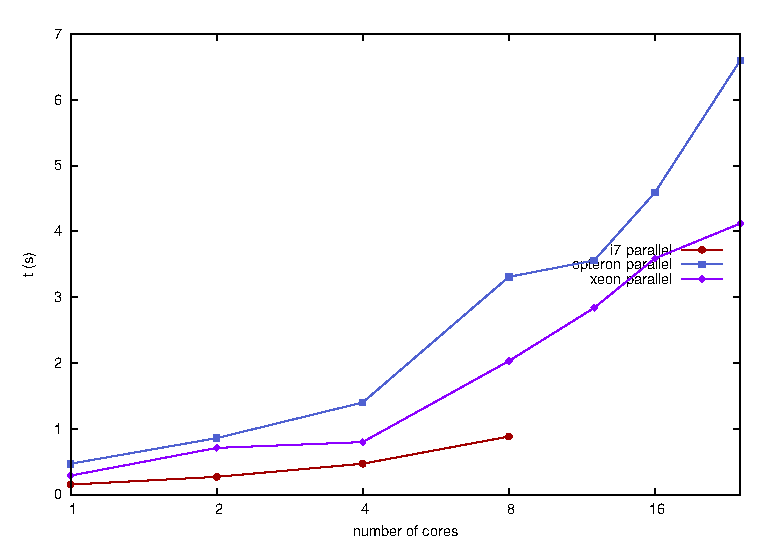
\includegraphics[width=10cm]{images/parallel.eps}
		\caption{Parallel section runtime}
		\label{fig:roofline}
	\end{figure}
	\end{center}
\end{frame}


\section{Roadmap}
\begin{frame}
	\begin{center}
	\begin{itemize}
		\item GPU version delayed;
		\item Thorough restructuring of the code;
	\end{itemize}
	\end{center}
\end{frame}

\section{Questions}
\begin{frame}
	\titlepage
	
	
\end{frame}

\end{document}%	end presentation